% SOURCE: edit-harness/results/frame_a/cells/cell_*_real_MIX_{A,B,C}_*.json + p2_llama-3.2-1b_real_MIX_C.json
% !TEX encoding = UTF-8 Unicode
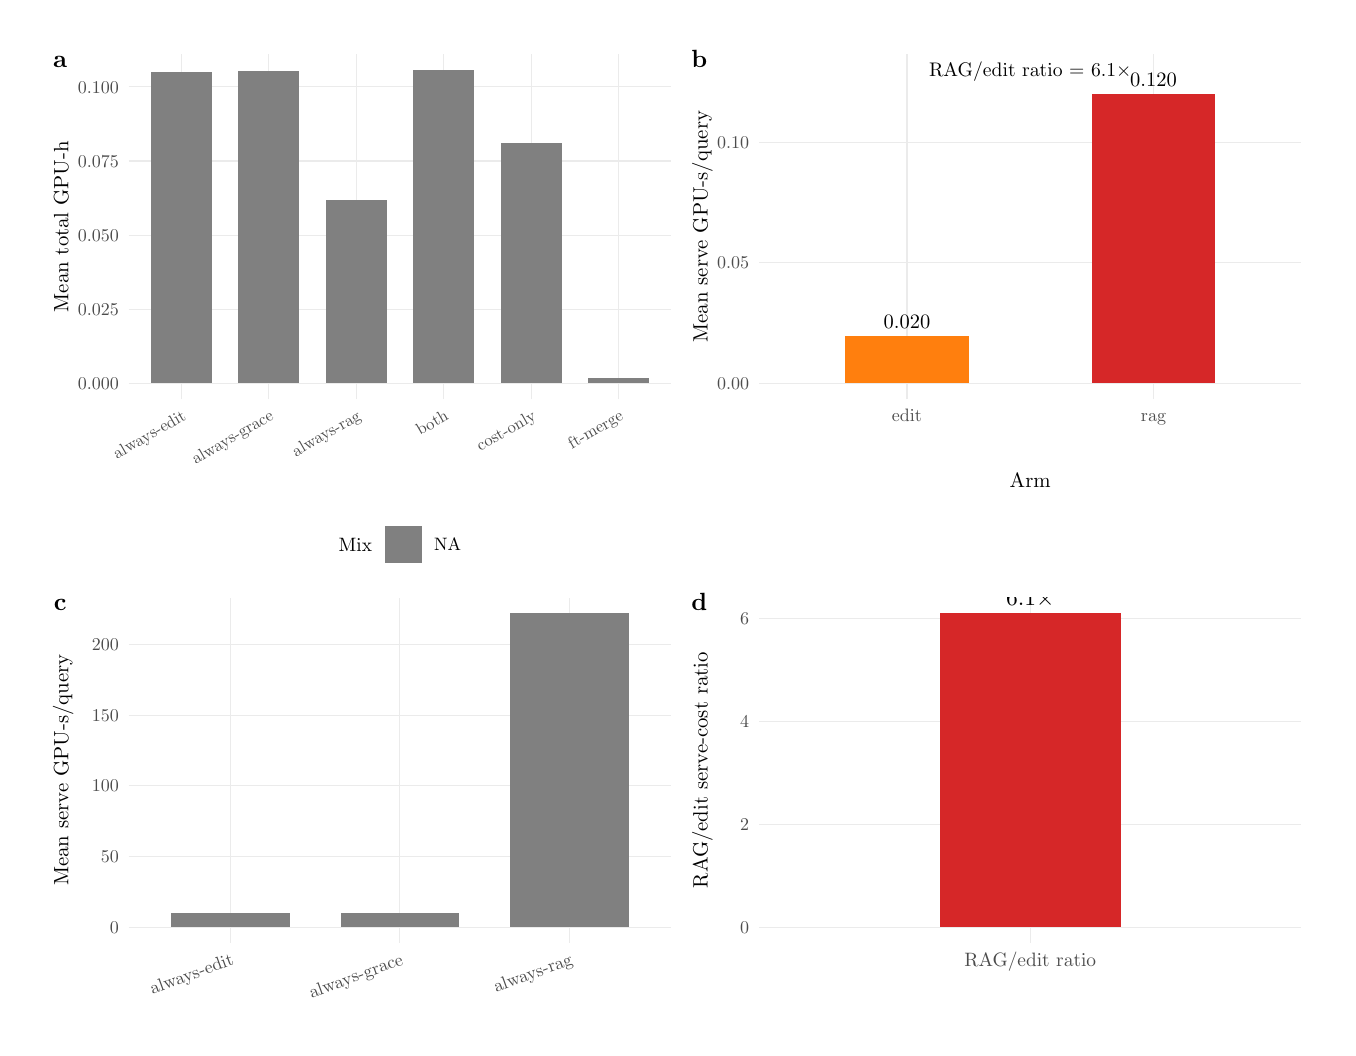
\begin{tikzpicture}[x=1pt,y=1pt]
\definecolor{fillColor}{RGB}{255,255,255}
\path[use as bounding box,fill=fillColor,fill opacity=0.00] (0,0) rectangle (469.75,361.35);
\begin{scope}
\path[clip] (  0.00,  0.00) rectangle (469.75,361.35);
\definecolor{drawColor}{RGB}{255,255,255}
\definecolor{fillColor}{RGB}{255,255,255}

\path[draw=drawColor,line width= 0.6pt,line join=round,line cap=round,fill=fillColor] (  0.00,  0.00) rectangle (469.76,361.35);
\end{scope}
\begin{scope}
\path[clip] (  5.50,159.41) rectangle (236.50,355.85);
\definecolor{fillColor}{RGB}{255,255,255}

\path[fill=fillColor] (  5.50,159.41) rectangle (236.50,355.85);
\end{scope}
\begin{scope}
\path[clip] (236.50,159.41) rectangle (464.25,355.85);
\definecolor{fillColor}{RGB}{255,255,255}

\path[fill=fillColor] (236.50,159.41) rectangle (464.25,355.85);
\end{scope}
\begin{scope}
\path[clip] (  5.50,  5.50) rectangle (236.50,159.41);
\definecolor{fillColor}{RGB}{255,255,255}

\path[fill=fillColor] (  5.50,  5.50) rectangle (236.50,159.41);
\end{scope}
\begin{scope}
\path[clip] (236.50,  5.50) rectangle (464.25,159.41);
\definecolor{fillColor}{RGB}{255,255,255}

\path[fill=fillColor] (236.50,  5.50) rectangle (464.25,159.41);
\end{scope}
\begin{scope}
\path[clip] ( 36.53,227.11) rectangle (232.50,351.85);
\definecolor{drawColor}{gray}{0.92}

\path[draw=drawColor,line width= 0.4pt,line join=round] ( 36.53,232.78) --
	(232.50,232.78);

\path[draw=drawColor,line width= 0.4pt,line join=round] ( 36.53,259.58) --
	(232.50,259.58);

\path[draw=drawColor,line width= 0.4pt,line join=round] ( 36.53,286.38) --
	(232.50,286.38);

\path[draw=drawColor,line width= 0.4pt,line join=round] ( 36.53,313.18) --
	(232.50,313.18);

\path[draw=drawColor,line width= 0.4pt,line join=round] ( 36.53,339.98) --
	(232.50,339.98);

\path[draw=drawColor,line width= 0.4pt,line join=round] ( 55.49,227.11) --
	( 55.49,351.85);

\path[draw=drawColor,line width= 0.4pt,line join=round] ( 87.10,227.11) --
	( 87.10,351.85);

\path[draw=drawColor,line width= 0.4pt,line join=round] (118.71,227.11) --
	(118.71,351.85);

\path[draw=drawColor,line width= 0.4pt,line join=round] (150.32,227.11) --
	(150.32,351.85);

\path[draw=drawColor,line width= 0.4pt,line join=round] (181.93,227.11) --
	(181.93,351.85);

\path[draw=drawColor,line width= 0.4pt,line join=round] (213.54,227.11) --
	(213.54,351.85);
\definecolor{fillColor}{gray}{0.50}

\path[fill=fillColor] ( 44.43,232.78) rectangle ( 66.55,299.91);

\path[fill=fillColor] ( 76.04,232.78) rectangle ( 98.16,300.98);

\path[fill=fillColor] (107.65,232.78) rectangle (129.77,288.34);

\path[fill=fillColor] (139.26,232.78) rectangle (161.38,299.51);

\path[fill=fillColor] (170.86,232.78) rectangle (192.99,292.24);

\path[fill=fillColor] (202.47,232.78) rectangle (224.60,234.54);

\path[fill=fillColor] ( 44.43,232.78) rectangle ( 66.55,293.78);

\path[fill=fillColor] ( 76.04,232.78) rectangle ( 98.16,298.29);

\path[fill=fillColor] (107.65,232.78) rectangle (129.77,298.91);

\path[fill=fillColor] (139.26,232.78) rectangle (161.38,296.61);

\path[fill=fillColor] (170.86,232.78) rectangle (192.99,289.81);

\path[fill=fillColor] (202.47,232.78) rectangle (224.60,234.76);

\path[fill=fillColor] ( 44.43,232.78) rectangle ( 66.55,345.31);

\path[fill=fillColor] ( 76.04,232.78) rectangle ( 98.16,345.52);

\path[fill=fillColor] (107.65,232.78) rectangle (129.77,266.87);

\path[fill=fillColor] (139.26,232.78) rectangle (161.38,346.18);

\path[fill=fillColor] (170.86,232.78) rectangle (192.99,319.76);

\path[fill=fillColor] (202.47,232.78) rectangle (224.60,234.69);
\end{scope}
\begin{scope}
\path[clip] (  0.00,  0.00) rectangle (469.75,361.35);
\definecolor{drawColor}{gray}{0.30}

\node[text=drawColor,anchor=base east,inner sep=0pt, outer sep=0pt, scale=  0.65] at ( 32.93,230.55) {0.000};

\node[text=drawColor,anchor=base east,inner sep=0pt, outer sep=0pt, scale=  0.65] at ( 32.93,257.34) {0.025};

\node[text=drawColor,anchor=base east,inner sep=0pt, outer sep=0pt, scale=  0.65] at ( 32.93,284.14) {0.050};

\node[text=drawColor,anchor=base east,inner sep=0pt, outer sep=0pt, scale=  0.65] at ( 32.93,310.94) {0.075};

\node[text=drawColor,anchor=base east,inner sep=0pt, outer sep=0pt, scale=  0.65] at ( 32.93,337.74) {0.100};
\end{scope}
\begin{scope}
\path[clip] (  0.00,  0.00) rectangle (469.75,361.35);
\definecolor{drawColor}{gray}{0.30}

\node[text=drawColor,rotate= 30.00,anchor=base east,inner sep=0pt, outer sep=0pt, scale=  0.60] at ( 57.56,219.94) {always-edit};

\node[text=drawColor,rotate= 30.00,anchor=base east,inner sep=0pt, outer sep=0pt, scale=  0.60] at ( 89.17,219.94) {always-grace};

\node[text=drawColor,rotate= 30.00,anchor=base east,inner sep=0pt, outer sep=0pt, scale=  0.60] at (120.78,219.94) {always-rag};

\node[text=drawColor,rotate= 30.00,anchor=base east,inner sep=0pt, outer sep=0pt, scale=  0.60] at (152.38,219.94) {both};

\node[text=drawColor,rotate= 30.00,anchor=base east,inner sep=0pt, outer sep=0pt, scale=  0.60] at (183.99,219.94) {cost-only};

\node[text=drawColor,rotate= 30.00,anchor=base east,inner sep=0pt, outer sep=0pt, scale=  0.60] at (215.60,219.94) {ft-merge};
\end{scope}
\begin{scope}
\path[clip] (  0.00,  0.00) rectangle (469.75,361.35);
\definecolor{drawColor}{RGB}{0,0,0}

\node[text=drawColor,rotate= 90.00,anchor=base,inner sep=0pt, outer sep=0pt, scale=  0.75] at ( 14.67,289.48) {Mean total GPU-h};
\end{scope}
\begin{scope}
\path[clip] (  0.00,  0.00) rectangle (469.75,361.35);
\definecolor{drawColor}{RGB}{0,0,0}

\node[text=drawColor,anchor=base west,inner sep=0pt, outer sep=0pt, scale=  0.70] at (112.39,172.23) {Mix};
\end{scope}
\begin{scope}
\path[clip] (  0.00,  0.00) rectangle (469.75,361.35);
\definecolor{fillColor}{gray}{0.50}

\path[fill=fillColor] (128.96,167.93) rectangle (142.38,181.35);
\end{scope}
\begin{scope}
\path[clip] (  0.00,  0.00) rectangle (469.75,361.35);
\definecolor{drawColor}{RGB}{0,0,0}

\node[text=drawColor,anchor=base west,inner sep=0pt, outer sep=0pt, scale=  0.65] at (146.89,172.40) {NA};
\end{scope}
\begin{scope}
\path[clip] (  0.00,  0.00) rectangle (469.75,361.35);
\definecolor{drawColor}{RGB}{0,0,0}

\node[text=drawColor,anchor=base,inner sep=0pt, outer sep=0pt, scale=  0.90] at ( 11.73,346.86) {\bfseries a};
\end{scope}
\begin{scope}
\path[clip] (264.28,227.11) rectangle (460.25,351.85);
\definecolor{drawColor}{gray}{0.92}

\path[draw=drawColor,line width= 0.4pt,line join=round] (264.28,232.78) --
	(460.25,232.78);

\path[draw=drawColor,line width= 0.4pt,line join=round] (264.28,276.40) --
	(460.25,276.40);

\path[draw=drawColor,line width= 0.4pt,line join=round] (264.28,320.01) --
	(460.25,320.01);

\path[draw=drawColor,line width= 0.4pt,line join=round] (317.73,227.11) --
	(317.73,351.85);

\path[draw=drawColor,line width= 0.4pt,line join=round] (406.81,227.11) --
	(406.81,351.85);
\definecolor{fillColor}{RGB}{255,127,14}

\path[fill=fillColor] (295.46,232.78) rectangle (340.00,249.95);
\definecolor{fillColor}{RGB}{214,39,40}

\path[fill=fillColor] (384.54,232.78) rectangle (429.08,337.53);
\definecolor{drawColor}{RGB}{0,0,0}

\node[text=drawColor,anchor=base,inner sep=0pt, outer sep=0pt, scale=  0.74] at (317.73,252.50) {0.020};

\node[text=drawColor,anchor=base,inner sep=0pt, outer sep=0pt, scale=  0.74] at (406.81,340.08) {0.120};

\node[text=drawColor,anchor=base,inner sep=0pt, outer sep=0pt, scale=  0.71] at (362.27,343.73) {RAG/edit ratio = 6.1$\times$};
\end{scope}
\begin{scope}
\path[clip] (  0.00,  0.00) rectangle (469.75,361.35);
\definecolor{drawColor}{gray}{0.30}

\node[text=drawColor,anchor=base east,inner sep=0pt, outer sep=0pt, scale=  0.65] at (260.68,230.55) {0.00};

\node[text=drawColor,anchor=base east,inner sep=0pt, outer sep=0pt, scale=  0.65] at (260.68,274.16) {0.05};

\node[text=drawColor,anchor=base east,inner sep=0pt, outer sep=0pt, scale=  0.65] at (260.68,317.77) {0.10};
\end{scope}
\begin{scope}
\path[clip] (  0.00,  0.00) rectangle (469.75,361.35);
\definecolor{drawColor}{gray}{0.30}

\node[text=drawColor,anchor=base,inner sep=0pt, outer sep=0pt, scale=  0.65] at (317.73,219.04) {edit};

\node[text=drawColor,anchor=base,inner sep=0pt, outer sep=0pt, scale=  0.65] at (406.81,219.04) {rag};
\end{scope}
\begin{scope}
\path[clip] (  0.00,  0.00) rectangle (469.75,361.35);
\definecolor{drawColor}{RGB}{0,0,0}

\node[text=drawColor,anchor=base,inner sep=0pt, outer sep=0pt, scale=  0.75] at (362.27,195.32) {Arm};
\end{scope}
\begin{scope}
\path[clip] (  0.00,  0.00) rectangle (469.75,361.35);
\definecolor{drawColor}{RGB}{0,0,0}

\node[text=drawColor,rotate= 90.00,anchor=base,inner sep=0pt, outer sep=0pt, scale=  0.75] at (245.67,289.48) {Mean serve GPU-s/query};
\end{scope}
\begin{scope}
\path[clip] (  0.00,  0.00) rectangle (469.75,361.35);
\definecolor{drawColor}{RGB}{0,0,0}

\node[text=drawColor,anchor=base,inner sep=0pt, outer sep=0pt, scale=  0.90] at (242.70,346.86) {\bfseries b};
\end{scope}
\begin{scope}
\path[clip] ( 36.53, 30.67) rectangle (232.50,155.41);
\definecolor{drawColor}{gray}{0.92}

\path[draw=drawColor,line width= 0.4pt,line join=round] ( 36.53, 36.34) --
	(232.50, 36.34);

\path[draw=drawColor,line width= 0.4pt,line join=round] ( 36.53, 61.88) --
	(232.50, 61.88);

\path[draw=drawColor,line width= 0.4pt,line join=round] ( 36.53, 87.41) --
	(232.50, 87.41);

\path[draw=drawColor,line width= 0.4pt,line join=round] ( 36.53,112.94) --
	(232.50,112.94);

\path[draw=drawColor,line width= 0.4pt,line join=round] ( 36.53,138.47) --
	(232.50,138.47);

\path[draw=drawColor,line width= 0.4pt,line join=round] ( 73.27, 30.67) --
	( 73.27,155.41);

\path[draw=drawColor,line width= 0.4pt,line join=round] (134.51, 30.67) --
	(134.51,155.41);

\path[draw=drawColor,line width= 0.4pt,line join=round] (195.76, 30.67) --
	(195.76,155.41);
\definecolor{fillColor}{gray}{0.50}

\path[fill=fillColor] ( 51.84, 36.34) rectangle ( 94.71, 39.90);

\path[fill=fillColor] (113.08, 36.34) rectangle (155.95, 39.71);

\path[fill=fillColor] (174.32, 36.34) rectangle (217.19,131.62);

\path[fill=fillColor] ( 51.84, 36.34) rectangle ( 94.71, 39.80);

\path[fill=fillColor] (113.08, 36.34) rectangle (155.95, 39.59);

\path[fill=fillColor] (174.32, 36.34) rectangle (217.19,149.74);

\path[fill=fillColor] ( 51.84, 36.34) rectangle ( 94.71, 41.35);

\path[fill=fillColor] (113.08, 36.34) rectangle (155.95, 41.54);

\path[fill=fillColor] (174.32, 36.34) rectangle (217.19, 94.79);
\end{scope}
\begin{scope}
\path[clip] (  0.00,  0.00) rectangle (469.75,361.35);
\definecolor{drawColor}{gray}{0.30}

\node[text=drawColor,anchor=base east,inner sep=0pt, outer sep=0pt, scale=  0.65] at ( 32.93, 34.11) {0};

\node[text=drawColor,anchor=base east,inner sep=0pt, outer sep=0pt, scale=  0.65] at ( 32.93, 59.64) {50};

\node[text=drawColor,anchor=base east,inner sep=0pt, outer sep=0pt, scale=  0.65] at ( 32.93, 85.17) {100};

\node[text=drawColor,anchor=base east,inner sep=0pt, outer sep=0pt, scale=  0.65] at ( 32.93,110.70) {150};

\node[text=drawColor,anchor=base east,inner sep=0pt, outer sep=0pt, scale=  0.65] at ( 32.93,136.24) {200};
\end{scope}
\begin{scope}
\path[clip] (  0.00,  0.00) rectangle (469.75,361.35);
\definecolor{drawColor}{gray}{0.30}

\node[text=drawColor,rotate= 20.00,anchor=base east,inner sep=0pt, outer sep=0pt, scale=  0.65] at ( 74.80, 22.87) {always-edit};

\node[text=drawColor,rotate= 20.00,anchor=base east,inner sep=0pt, outer sep=0pt, scale=  0.65] at (136.04, 22.87) {always-grace};

\node[text=drawColor,rotate= 20.00,anchor=base east,inner sep=0pt, outer sep=0pt, scale=  0.65] at (197.29, 22.87) {always-rag};
\end{scope}
\begin{scope}
\path[clip] (  0.00,  0.00) rectangle (469.75,361.35);
\definecolor{drawColor}{RGB}{0,0,0}

\node[text=drawColor,rotate= 90.00,anchor=base,inner sep=0pt, outer sep=0pt, scale=  0.75] at ( 14.67, 93.04) {Mean serve GPU-s/query};
\end{scope}
\begin{scope}
\path[clip] (  0.00,  0.00) rectangle (469.75,361.35);
\definecolor{drawColor}{RGB}{0,0,0}

\node[text=drawColor,anchor=base,inner sep=0pt, outer sep=0pt, scale=  0.90] at ( 11.73,150.85) {\bfseries c};
\end{scope}
\begin{scope}
\path[clip] (264.28, 30.67) rectangle (460.25,155.41);
\definecolor{drawColor}{gray}{0.92}

\path[draw=drawColor,line width= 0.4pt,line join=round] (264.28, 36.34) --
	(460.25, 36.34);

\path[draw=drawColor,line width= 0.4pt,line join=round] (264.28, 73.51) --
	(460.25, 73.51);

\path[draw=drawColor,line width= 0.4pt,line join=round] (264.28,110.68) --
	(460.25,110.68);

\path[draw=drawColor,line width= 0.4pt,line join=round] (264.28,147.85) --
	(460.25,147.85);

\path[draw=drawColor,line width= 0.4pt,line join=round] (362.27, 30.67) --
	(362.27,155.41);
\definecolor{fillColor}{RGB}{214,39,40}

\path[fill=fillColor] (329.60, 36.34) rectangle (394.93,149.74);
\definecolor{drawColor}{RGB}{0,0,0}

\node[text=drawColor,anchor=base,inner sep=0pt, outer sep=0pt, scale=  0.85] at (362.27,152.68) {6.1$\times$};
\end{scope}
\begin{scope}
\path[clip] (  0.00,  0.00) rectangle (469.75,361.35);
\definecolor{drawColor}{gray}{0.30}

\node[text=drawColor,anchor=base east,inner sep=0pt, outer sep=0pt, scale=  0.65] at (260.68, 34.11) {0};

\node[text=drawColor,anchor=base east,inner sep=0pt, outer sep=0pt, scale=  0.65] at (260.68, 71.28) {2};

\node[text=drawColor,anchor=base east,inner sep=0pt, outer sep=0pt, scale=  0.65] at (260.68,108.44) {4};

\node[text=drawColor,anchor=base east,inner sep=0pt, outer sep=0pt, scale=  0.65] at (260.68,145.61) {6};
\end{scope}
\begin{scope}
\path[clip] (  0.00,  0.00) rectangle (469.75,361.35);
\definecolor{drawColor}{gray}{0.30}

\node[text=drawColor,anchor=base,inner sep=0pt, outer sep=0pt, scale=  0.70] at (362.27, 22.25) {RAG/edit ratio};
\end{scope}
\begin{scope}
\path[clip] (  0.00,  0.00) rectangle (469.75,361.35);
\definecolor{drawColor}{RGB}{0,0,0}

\node[text=drawColor,rotate= 90.00,anchor=base,inner sep=0pt, outer sep=0pt, scale=  0.75] at (245.67, 93.04) {RAG/edit serve-cost ratio};
\end{scope}
\begin{scope}
\path[clip] (  0.00,  0.00) rectangle (469.75,361.35);
\definecolor{drawColor}{RGB}{0,0,0}

\node[text=drawColor,anchor=base,inner sep=0pt, outer sep=0pt, scale=  0.90] at (242.70,150.85) {\bfseries d};
\end{scope}
\end{tikzpicture}
